\documentclass[12pt]{article}
\usepackage[a4paper, total={6in, 8in}]{geometry}
\usepackage[utf8]{inputenc}
\usepackage[english]{babel}
\usepackage{titlesec}
\usepackage{graphicx}
 

\usepackage{setspace}
\doublespacing


%   Thesis / research paper title.
%	Student name, student number.
%	Date.
%	Keywords: 2 on concepts, 2 on methods, 1 on the field of observation.
%	Department, University.


\title{ }
\author{Berthin Bitja \\ 4532321}
\date{}



\usepackage[
style=nature,
date=year,
backend=biber,
natbib=true,
doi=false,
defernumbers=true
]{biblatex}


\graphicspath{{_img/}} %Folder with img
\frenchspacing % only one space between sentences


\usepackage{lineno} %add number to every line
\linenumbers

\addbibresource{bib-influenza.bib}

\begin{document}

\begin{titlepage}
	\centering

	{\Large\bfseries Deep learning approaches for forecasting the global spread of influenza \par}
	\vspace{2cm}
	{\small Berthin Bitja \\ 4532321 \par}
	{\small \today\par}
	\vfill
	
	{\large Department of Biology \\ University of Ottawa \par}

% Bottom of the page

\end{titlepage}

\newpage

\tableofcontents

\newpage

\section{Introduction}
Influenza is a recurrent public health problem. The virus infects approximately $5\%$ of the global adult population and $20\%$ of children every year causing respiratory illness and complications\autocite{Ting2017}. In Canada, the total cost of each influenza season is estimated to 1 billion per year\autocite{Molinari2007}. In additon, new influenza variants arise every year due to virus re-assortment (i.e. mixing of genetic material) and the accumulation of mutations. Nevertheless, most of these variants are not harmfull to human population. As a result, public health agencies and government set up preventive programs  to restrain infection and widespread transmission of circulating strains\autocite{Jefferson2005}.In order to complete this task, 

This research leverage the technology advances in computing power, machine-learning and the abundance of data on influenza epidemiology and genetic, climate and human mobility, in order to utilize new class of machine learning methods named deep learning (DL) , to predict potential epidemic areas worldwide.

\section{Background}

\subsection{Influenza forecasting method}

In the recent years, several  methods to forecast influenza outbreak have been reported\autocite{nsoesie2014}. Time-series models are among the most popular, especially  autoregressive integrated moving average (ARIMA) models. The ARIMA models assume that future values can be predicted based on past observations\autocite{quenel1998}. The ARIMA models is capable of capturing trend and periodic changes relationship. However, influenza activity varies from season to season, outbreaks can occur off-season. In an attempt to account for this type of irregularities, methods of analogs match current influenza patterns to patterns of historical outbreaks\autocite{viboud2003}. Although, they perform better than ARIMA models, these models are limited to the sensitivity to forecasts and the difficulty to find patterns due to the irregularity of historical outbreaks. Compartmental models include the effect of human behaviour by dividing the population into sub-populations according to the state of the disease and defining the rate at which individuals move between sub-populations. Although the model present simple and well studied behaviour it fails to capture the differences in contact patterns for different age groups and environments\autocite{degli2008}. More complex model such as agent-based models study global behavior related to interactions of defined individual entities (agents) within a define environment \autocite{carrasco2013}. In contrast, metapopulation models divide populations in separated and discrete habitat areas and sub-populations, where populations interact through migration. The model describes the dynamics within areas, trough define disease states, and uses mobility networks to simulate the diffusion patterns of an ongoing epidemic. Agent based models and metapopulation models have been used to evaluate the effectiveness of various measures for controlling influenza epidemics. The main constrains of these models are the lack of empiric evidence to justify the modeling suppositions and defining parameters\autocite{nsoesie2014}.


\subsection{Deep Learning and influenza}
A deep-learning architecture is a multilayer stack of artificial neurons computing non-linear input–output mappings. Each artificial neurons in the stack transforms its input to increase both the selectivity and the invariance of the representation\autocite{leCun2015}. The key advantage of Artificial Neural Networks (ANN) is the possibility for the model to automatically learn good features to evaluate the input. The backpropagation procedures train the model by computing partial derivatives of the objective function with respect to the weight and threshold coefficients. Deep learning offers different types of architectures : Convolutional Neural Network (CNN) for computer vision problem, and Reccurent Neural Networks (RNN) to process sequencial input, such as speech and languange\autocite{leCun2015, Miotto2017}. 
 
 Disease transmission is a complex geo-temporal that includes environment factors\autocite{Pica2012} such as temperatures, humidity or pressure, genomic information such as drug resistant mutations, and human behavior that can be represented by airport traffic. In addition, these type of data constitute large datasets. In this context, DL offers an alternative approach to resolve prediction problems by enabling computational models that are composed of multiple processing layers based on ANN to learn representations of data with multiple levels of abstraction. Those ``black boxes'' reduce the need for feature engineering considering that features are learned from data. Despite, being used in various fields such as speech recognition, visual object recognition, object detection, drug discovery and genomics, there are no publicly available tools implementing these algorithms for the forecasting of influenza outbreaks.

\section{Goal}

The goal of this thesis is to predict areas where we observe influenza activities at the local, regional, national, or global level by implementing a DL. The underlying objectives of this thesis are (i) to design the architecture of a deep neural network integrating human mobility data, genomic data and environmental data to predict common epidemic measures \autocite{nsoesie2014} including locations,  period and activity level of the different types and subtypes of influenza,  (ii) to develop a pipeline to automate the data retrieval process, (iii) to assess the overall performance of our design and (iv) to benchmark our DL design against published influenza forecasting methods . The motivation of this research is to expand the knowledge on predictive methods based on DL approaches for surveillance and forecasting of infectious diseases and explores the relevance of using DL in application to influenza forecasting. 

\section{Methodology}

\begin{figure}[h]
    \centering
    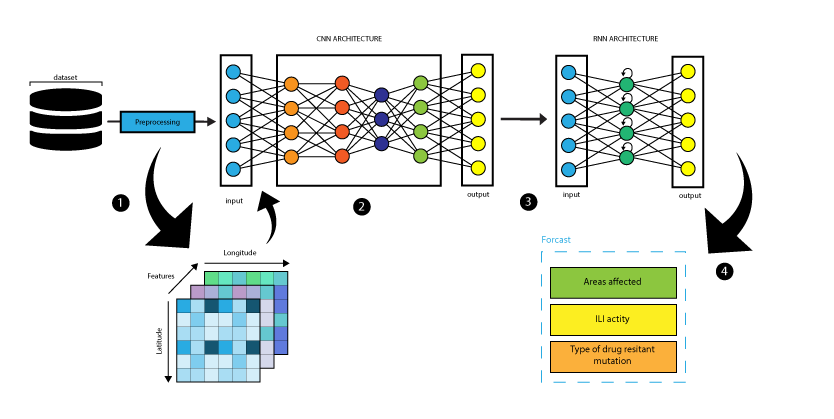
\includegraphics[width=\textwidth]{figure-1.png}
    \caption{\textbf{Predicting influenza activity.}  The output (4) is generated by a recurrent neural network (RNN) taking, as input, the representation  (3)  extracted by a deep (2) convolution neural network (CNN) from  (1) 3-D representation input obtained from preprocessing the different datasets, with the RNN trained to produce prediction based on the high-level representations of the data}
    \label{fig:model}
\end{figure}

We are going to explore a method based on the combination of a CNN and RNN (Fig.\ref{fig:model}). The CNN is used to embedded representation of the virus according to its location at a specific time step. Then the CNN output is given to the RNN to produce a prediction. 


\subsection{Data acquisition}
 In order for the data to become an input for our computational graph, it need to be transformed into a tensor. In CNN, features represent channels, each channel form as 2-D array where the rows represent intervals of latitudes, the columns represent interval of longitudes and the cell represent the number of observation of the virus (Fig.\ref{fig:model}). The parameters we are going to use for this model are obtained from the Influenza Virus Database\autocite{chang2006influenza} for genomic information, Global Surface Summary of the Day (GSOD)\autocite{Lott1998} database for environmental factors, FluNet database\autocite{flahault1998} for virus infectivity and the Bureau of Transportation Statistics database\autocite{mcdonald2013} for host behavior. To simplify the data processing, we are going to represent the features as discrete variable. For example, climate factor are going to be represented as interval of temperature, pressure and humidity. This process will reduce the size of our input.
 
\subsection{Convolutional Neural Networks}
CNN are a type of neural networks specialized for processing data  that has know grid-like topology (Fig.\ref{fig:model}). The common application of CNN architecture is for the classification of image inputs. The layers of a CNN have neurons arranged in 3-D, width, height, depth (here depth refers to channels). To build a CNN architecture we need three main types of layers : Convolutional Layer, Pooling Layer, and Fully-Connected Layer.

A typical CNN architecture contains :
\begin{itemize}
\item \textbf{Input layer} that holds the raw values of the data, in our case the representation of influenza over 360° of longitude (as width),  and 180° of latitude (as height), and with features representing our channels.
\item \textbf{Convolutional layer} that computes the output of neurons that are connected to local regions in the input. 
\item \textbf{ReLU layer} applies an elementwise activation function, such as the $max(0,x)max(0,x)$ thresholding at zero.
\item \textbf{Pooling layer} performs a downsampling operation along the spatial dimensions (width, height), resulting in a smaller volume.
\item \textbf{Fully-connected layer} computes the class scores, where each of the labels correspond to a class score.
\end{itemize}
CNN transform the 3-D representation of the data, layer by layer, from the quantitative values to the final class scores. In CNN, parameters are not shared trough every layers. In particular, the convolutional/fully-connected layers perform transformations that are a function of not only the activations in the input volume, but also of the parameters (the weights and biases of the neurons). On the other hand, the ReLU/Pooling layers will implement a fixed function. The parameters in the convolutional/fully-connected layers will be trained trough backpropagation so that the class scores that the CNN computes are consistent with the labels in the training set for each representation of our data.

\subsection{Reccurent Neural Networks}
To produce a forcast we need to be able to accumulate knowledge over time. Although, CNN can share parameters across time but it lacks depth. The convolution process compute the output from a small number of neighboring members of the previous layer. In the case of RNN, each layer uses the same update from the previous layer. Subsequently, parameters in RNN are shared trough the deep computational graph (Fig.\ref{fig:RNN}).

We define the input obtained from our CNN, $p$, that varies trough discrete time step, $t$, to give an output, $o$. The state, $s$, of the system is defined by :
$$s_t = f(Up_t+ Ws_{t-1})$$ where $(U,W)$ are parameters of the RNN (Fig.\ref{fig:RNN}). The activation function $f$ is a non-linear function that transform the input from the previous layer to a new output for the next layer. Each observations, $o_{t=0,1,2 ... }$ depends on the computed knowledge we have on the profile of the virus. The prediction or observations, $o_t$, can be produced trough a vector of probabilities  $$o_t=softmax(Vs_t)$$ where, $V$, represent the features of our virus representation. $Softmax$ function calculates the probabilities distribution, $P$, over discrete states $P(s_t)$ .

\begin{figure}[h]
    \centering
    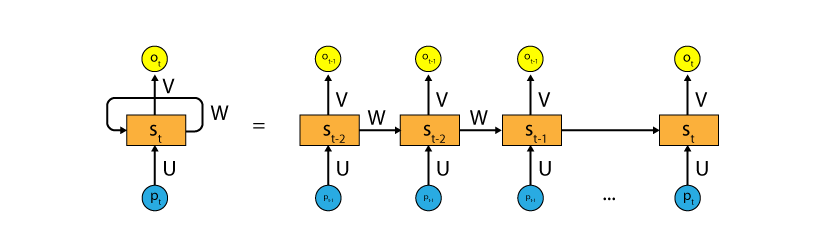
\includegraphics[width=\textwidth]{figure-3.png}
    \caption{ \textbf{An unrolled recurrent neural network.} The artificial neurons (for example, hidden units grouped under node s with values $s_t$ at time t) get inputs from other neurons at previous time steps. In this way, a recurrent neural network can map an input sequence with elements $s_t$ into an output sequence with elements $o_t$, with each $o_t$ depending on all the previous $p'_t$ (for $t'\leq t$). The same parameters (matrices $U,V,W$ ) are used at each time step. }
    \label{fig:RNN}
\end{figure}

\subsection{Implementation, training and testing}

We are going to implement the architecture of our neural network using Tensorflow\autocite{abadi2016} as the framework. This is an open source library for fast numerical computing. This framework allows to build efficient series of matrix transforms in a format intended to be executed on graphics processing unit (GPU) or central processing unit (CPU). 

To train our neural network, we perform cross-validation methods. The data is randomly split into 3 types of set: (i) training set to adjust the weights trough gradient descent; (ii) validation set to tune the hyperparameters such as the initial learning rate, learning rate decay or regularization strength (Loss function); (iii) test set to assess the performance of the data, such as the accuracy, precision and the sensitivity. 

\section{Timeline}

\begin{figure}[h]
    \centering
    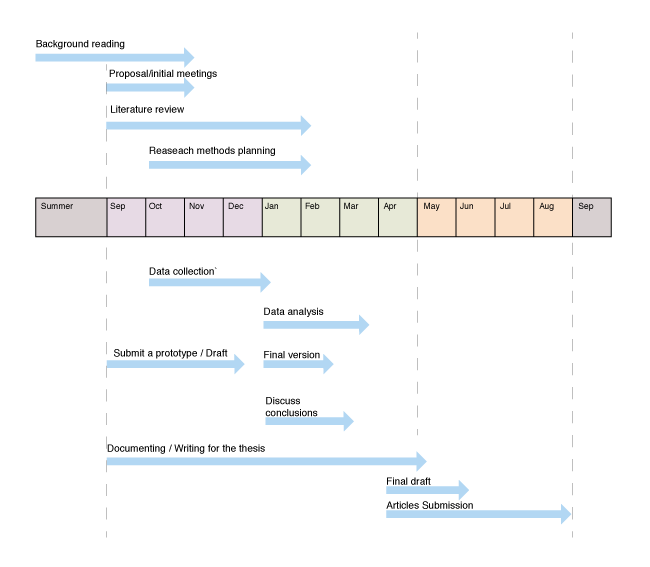
\includegraphics[width=\textwidth]{figure-2.png}
    \caption{ \textbf{Timeline for the completion of the research.} The implementation of the Deep learning is divided in 4 phases : data acquisition, coding, training and evaluation of the models. The data acquisition and coding should be done by the end of February. The training and evaluation of the models should be done by the end of May.}
    \label{fig:plan}
\end{figure}

From September to December, we will perform the analysis and preprocessing of the input data on which the algorithm(s) will be applied. We will also extend our knowledge on the different theoretical structures on computational graph. Also, we will start writing the mathematical foundations for our neural network architecture, techniques and algorithms (Fig.\ref{fig:plan}). 

From October to May, we will be implementing our computational model. By mid October, we will finish coding the preliminary version of our deep learning model(s). Beetween January and May, we will finish coding, training and tuning the final version of the Deep Learning algorithm(s), and will evaluate the performance of the implemented algorithm(s) against existing implementations. Also during that period, we will start writing of the preliminary version of the thesis (Fig.\ref{fig:plan}).

In May, we expect finishing final draft of the thesis. At that time we will start the preparation of the seminar presentation, thesis defence, progress report presentation. We will finish writing the final version of the article and selected a list of scientific journal to apply. By the end of august we will have created of the slides for the thesis presentation, set the date for a the oral thesis defence (Fig.\ref{fig:plan}). 

\printbibliography[title={Bibliography},nottype=misc,resetnumbers=true]

\end{document}
